\documentclass{ximera}

%\graphicspath{{./}{eulerCharacteristic}}


\title{Euler Characteristic}	
\begin{document}
\begin{abstract}
In this activity we are going to investigate some fundamental
properties of shapes in different dimensions.
\end{abstract}
\maketitle

\section*{Data and Observations}

\paragraph{First Table}

\begin{question}
Consider the following shapes.
\begin{image}
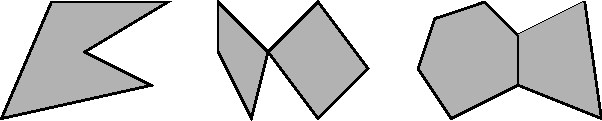
\includegraphics{eulerCharPoly.pdf}
\end{image}
For each shape, record the number of vertices, the number of edges,
and the number of faces in a table (does it appear?):
\begin{center}
\begin{tabular}{c|c|c}
Vertices & Edges & Faces\\
\hline\hline
 $\vdots$  & $\vdots$  & $\vdots$  \\ 
\end{tabular}
\end{center}
\end{question}

\begin{question}
Draw ten more shapes made from polygons. Record their number of
vertices, number of edges, and number of faces in your table too.
\begin{freeResponse}
\end{freeResponse}
\end{question}

\begin{problem}
Play around with this idea for a bit. Come up with as many questions
as you can and list them.
\begin{freeResponse}
\end{freeResponse}
\end{problem}

\begin{problem}
As a class, decided one (or more) of these problems to
investigate. Reflect upon the investigation and give a solution (if
you have one).
\begin{freeResponse}
\end{freeResponse}
\end{problem}





\end{document}









\begin{question}
Can \textit{any} set of three numbers appear in your table? Or is
there some rule telling you when a set of numbers is possible? 
\end{question}



\paragraph{Second Table}

\begin{question}
What if your shapes are disconnected? For example this is one shape:
\begin{image}
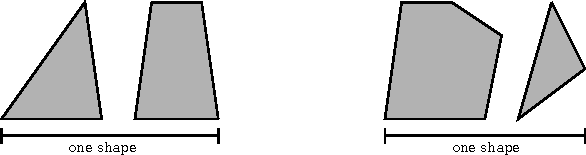
\includegraphics{eulerCharPoly2.pdf}
\end{image}
Draw five examples of disconnected shapes made from polygons. Record
their number of vertices, number of edges, number of faces, and pieces in a new
table:
\begin{center}
\begin{tabular}{c|c|c|c}
Vertices & Edges & Faces & Pieces\\
\hline\hline
 $\vdots$  & $\vdots$  & $\vdots$  & $\vdots$  \\ 
\end{tabular}
\end{center}
\end{question}

\begin{question}
Can \textit{any} set of four  numbers appear in your table? Or is
there some rule telling you when a set of numbers is possible? 
\end{question}


\paragraph{Third Table}


\begin{question}
What if your shapes have holes? For example, consider:
\begin{image}
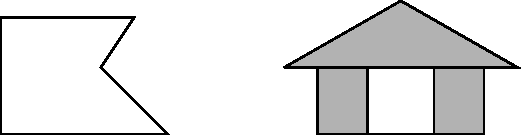
\includegraphics{eulerCharPoly3.pdf}
\end{image}
Draw five examples of shapes made from polygons with holes. Record
their number of vertices, number of edges, number of faces, and holes in a new
table:
\begin{center}
\begin{tabular}{c|c|c|c}
Vertices & Edges & Faces & Holes\\
\hline\hline
 $\vdots$  & $\vdots$  & $\vdots$  & $\vdots$  \\ 
\end{tabular}
\end{center}
\end{question}

\begin{question}
Can \textit{any} set of four numbers appear in your table? Or is
there some rule telling you when a set of numbers is possible? 
\end{question}


\paragraph{Fourth Table}

\begin{question}
Consider the Platonic solids and the triangular dipyramid. For these,
record the number of vertices, edges, and faces in a table.
\end{question}


\begin{question}
Can \textit{any} set of three numbers appear in your table? Or is
there some rule telling you when a set of numbers is possible? 
\end{question}



\section*{The Why and The How}


\begin{question}
Draw your favorite shape built from polygons in the plane---for fun,
make sure it has at least one non-triangular face. Compute
$V-E+F$. Explain why this number doesn't change when:
\begin{enumerate}
\item If there is a face that is not triangular, you add edges (but not vertices) to break it into triangles. 
\item If you remove a triangle on the outer border of your shape. Note that there are three cases to consider!
\end{enumerate}
\end{question}

\begin{question}
Use your work above to explain your observations for $V-E+F$ for
shapes made of polygons. Can you extend your argument to work for: 
\begin{itemize}
\item Shapes that are disconnected? 
\item Shapes that have holes?
\item Polyhedra? Hint: Use a sphere.
\end{itemize} 
\end{question}



\section*{Into the Wild}

\begin{question}
Consider the hypercube and the hypertetrahedron. Record the number of
vertices, edges, faces, and solids. Now compute: $V-E+F-S$. What do
you notice? Make wild conjectures and tell us about them.
\end{question}


\end{document}
